\chapter{Measurement Setup \& Techniques} \label{chapter:measurement}

In this chapter we discuss the measurement setup and techniques that we use in this thesis work. We present all individual parts of our signal generation and measurement chain, putting emphasis on the generation and measurement of high-frequency signals. Afterwards we briefly discuss the calibration and compensation techniques that we use to correct signal imperfections when generating qubit drive and flux signals. Finally we introduce the different measurement techniques that we use in this work, including qubit readout and driving as well as more advanced methods used to obtain all relevant qubit parameters such as frequency, anharmonicity as well as relaxation and dephasing times.

\smallskip

Our experimental setup consists of the qubit chip discussed in chapter \ref{chapter:design}, which is put at the 20 mK stage of a He$_3$/He$_4$ dilution cryostat and connected to a room temperature signal generation and measurement chain via cryogenic microwave components and 50 $\Omega$ coaxial transmission lines. At room temperature, we generate microwave pulses as well as DC and high-frequency flux bias pulses using heteordyne mixing and/or high-frequency arbitrary signal generators. We use a cryogenic amplifier chain and homodyne demodulation at room temperature to perform reflectometric measurements of the phase of our microwave readout signal.

\section{Sample Holder \& PCB}

\begin{SCfigure}[1][ht!]
	\centering
		\includegraphics[width=0.6\textwidth]{"./material/photos/sample holder/sample_holder"}
	\caption[]{The sample holder with the mounted PCB carrying the qubit chip. Bond wires are used to connect the on-chip tranmission lines to the PCB, which in turn uses a Mini-SMP connector to connect the bondwire to a set of external coaxial SMP cables. The top part of the sample holder is screwed to the bottom part, forming a closed box with cavities only for the tranmission lines and the qubit chip. The whole sample holder is screwed to the 20 mK stage of the dilution cryostat.}
	\label{fig:pcb_and_sample_holder}
\end{SCfigure}

For mounting the qubit chip as shown in fig. \ref{fig:qubit_chip_photos} in the sample holder, the chip is first glued to a custom-designed high-frequency PCB, as shown in fig. \ref{fig:pcb_and_sample_holder} (bottom). On this PCB, six 50 $\Omega$ CPW waveguides terminated by Mini-SMP connectors are bond-wired to the drive/readout and fast flux lines of the qubit chip. For each qubit, we have one readout/drive line and two flux lines on the chip. In addition, bond wires are used to connect the ground plane of the chip to that of the PCB. On-chip bond wires are used to connect separated parts of the on-chip ground plane which are isolated from each other due to the circuit topology. This is important in order to avoid spurious on-chip resonances in the relevant frequency range between $4-7$ GHz \citep{schuster_circuit_2007}. The PCB with the mounted chip is then screwed to a sample holder machined in copper that fully encloses the PCB, as shown in fig. \ref{fig:pcb_and_sample_holder} and that consists of a bottom part on which the PCB is screwed and that is itself screwed to the top part of the sample holder. The top part provides holes for the SMP connectors and is pressed against the surface of the PCB. Machined grooves in the top part provide the necessary open space above the qubit chip and the transmission lines on the PCB. The function of the sample holder is to thermally anchor the PCB and the qubit chip to the cryostat and, more importantly, to shield the qubit chip from spurious electromagnetic signals and enclose it in a conducting cavity that is small enough to suppress box resonances at all relevant working frequencies.

\section{Signal Generation \& Acquisition}

\begin{figure}[ht!]
	\centering
		\includegraphics[width=1.\textwidth]{"./material/figures/2-qubit-processor/measurement setup"}
	\caption[The measurement setup used for the two-qubit experiments]{The measurement setup used for the two-qubit experiments. Exactly the same drive and readout scheme is used for both qubits with phase-locked microwave sources and arbitrary waveform generators.}
	\label{fig:measurement_setup}
\end{figure}

Fig. \ref{fig:measurement_setup} shows the wiring of our experiment from room temperature down to the 20 mK state of the dilution cryostat. Superconducting cables are used where adequate to minimize signal attenuation, in addition lossy cables made from special alloys such as CuNi are used to minimize heat transfer into the cryostat, which is especially critical between the 300 mK and 20 mK stages. Pairs of bifilar cables are used to provide DC biasing of one or several superconducting coils.

\subsection{Driving and Measurement of the Qubit}

Each of the qubits together with its corresponding readout resonator on our chip is fitted with an individual drive and readout circuit. At room temperature we generate qubit and resonator drive waveforms using phase-locked single-tone microwave sources whose continous output is mixed with fast control pulses, that are generated by two arbitrary waveform generators (the details of this microwave mixing will be discussed in the following paragraph). The drive and readout signals are then combined and sent to the qubit chip through a series of (cryogenic) attenuators and filters. A cryogenic circulator at the 20 mK sample stage of the dilution cryostat routes the incoming pulses to the qubit chip, where they are sent to the qubit readout resonator and finally reflected by it. The reflected signal passes again through the input microwave circulator and gets routed through a double isolator and a band-pass filter to a cryogenic HEMT amplifier with a gain of 40 dB. The amplified signal gets then transmissted to the room temperature electronics, where it is filtered and amplified further. Finally, the signal is demodulated with a continous microwave reference tone and fed to an ADC board through a pair of low-noise amplifiers.

\smallskip

In addition to this, each qubit is equipped with a pair of fast flux lines. High-frequency and DC flux pulses are generated using an arbitrary waveform generator at room temperature. The flux signal is then sent to the qubit chip through 20 dB of attenuation, a conventional Microtronics low-pass filter as well as a custom-made high-frequency powder filter that uses an absorptive material (Eccosorb) to attenuate high-frequency noise. After passing through the transmission line on the qubit chip, the outgoing flux signal gets routed to room temperature through a tranmission line identical to the input line. There, the signal can be measured, which is useful for characterizing possible signal imperfections caused by the non-ideal character of the tranmsission line.

\subsection{Microwave Sideband Mixing}

To generate the qubit drive pulses we use single-sideband mixing techniques. We use a pair of IQ mixers that we drive with a continous single-frequency microwave tone and two synchronized fast control signals generated by an arbitrary waveform generator (Tektronix AWG5014b). In general, when feeding a signal $LO(t) = i_0 \cos{(\omega_{LO} t )}$ to the LO port of an IQ mixer and two signals $I(t)$, $Q(t)$ to the I and Q ports of the mixer, we obtain a signal

\begin{equation}
RF(t) = I(t)\cos{(\omega_{LO} t)}+Q(t)\sin{(\omega_{LO} t)} \label{eq:iqMixer}
\end{equation}

at the RF port of the mixer. Since the IQ mixer that we use is a passive, reciprocal device one can as well feed two input signals to the LO and RF ports and obtain the demodulated signal quadratures at the I and Q ports, a technique that we make use of in our qubit readout scheme. Typically we use heterodyne sideband mixing to generate drive pulses that are displaced in frequency in respect to the original LO (carrier) waveform.

\begin{figure}[ht!]
	\centering
		\includegraphics[width=0.7\textwidth]{"./material/figures/measurement/mixer_imperfections"}
	\caption[...]{Illustration of the method used to measure and correct the imperfect signal behavior of the IQ mixer used in our experiments: To minimize the leakage of the LO signal to the RF port, we apply a continous input signal at frequency $\omega_{LO}$ to the LO port and minimize the power at $\omega_{LO}$ the RF port, as measured by a fast spectrum analyzer, by tuning the two offset voltages $I_0$ and $Q_0$ at the IF1/I and IF2/Q ports. To correct phase and amplitude errors during heterodyne mixing, we apply the same signal as before to the LO port and in addition two sideband signals to the IF ports. We then minimize the measured power at the RF port at $\omega_{LO}+\omega_{IF}$ by adding a correction waveform at the IF ports.}
	\label{fig:iq_mixer_correction}
\end{figure}

Commercially available IQ mixers often deviate from the ideal behavior as given by eq. (\ref{eq:iqMixer}). Typical imperfections include large insertion losses --i.e. loss of signal power between the different ports of the mixer--, RF signal leakage at zero IQ-input and frequency-dependent phase and amplitude errors of the mixed sideband signals. In order to achieve reliable single-qubit operations we need to correct the signal leakage and quadrature-specific amplitude and phase errors. The signal leakage causes a small part of the LO signal to leak through to the RF port even when the IQ inputs are zeroed. This leakage can be compensated by adding LO frequency $\omega_{LO}$ dependent DC offset voltages to the IQ ports. The appropriate offset voltages can be determined by applying a continuous input signal at a frequency $\omega_c$ to the LO port of the mixer and minimizing the measured signal power at the RF port by varying the IQ offset voltages. To correct the sideband amplitude and phase errors we apply another correction procedure that we outline here. First, for the signals at the IQ inputs of the mixer we introduce the notation

\begin{equation}
A(t) = I(t)+iQ(t) = a(t)\exp{(-i\phi(t))} \label{eq:iq_if_input}
\end{equation}

We consider an IQ signal at a single sideband frequency $\omega_{IF}$ and at fixed complex amplitude $a(t) = a = a_0\exp{(i\phi_0)}$ such that $A(t) = a\exp{(-i \omega_{IF} t)}$. The effect of the gain and phase imperfections of the IQ mixers can then be modeled by assuming that the mixer adds another IQ signal $\epsilon(\omega_{IF},\omega_{LO})A^*(t)$ at the mirrored sideband frequency $-\omega_{IF}$. We can correct this unwanted signal by adding a small correction $c(\omega_{IF},\omega_{LO})A^*(t)$ to our IQ input signal. The complex-valued correction coefficient $c(\omega_{IF},\omega_{LO})=|c|\exp{(i\angle c)}$ usually depends both on the LO frequency $\omega_{LO}$ and the sideband frequency $\omega_{IF}$. We determine the correction coefficients by generating a continuous waveform at a given center and sideband frequency, measuring the amplitude of the unwanted sideband signal with a fast spectrum analyzer and minimizing its amplitude by varying the correction coefficient $c(\omega_{IF},\omega_{LO})$.

Both the offset and the sideband-amplitude and -phase corrections have been automated using our data acquisition software. By using the optimization techniques described above we can achieve $\le-80\;\mathrm{dBm}$ residual leakage power at the RF port of the mixer when no input IQ signal is present and a supression of the unwanted mirror sideband during heterodyne modulation by $>70\;\mathrm{dB}$.

\subsection{Fast Magnetic Flux Pulses}

We use a pair of superconducting coaxial cables to realize the qubit flux lines. Each qubit is connected to an on-chip transmission line, whose ends are connected to two fully symmetric transmission lines through the PCB. These two lines lead back to the room-temperature stage and can be used to send signals down the flux line and measure the transmitted signal. Between room temperature and the 20 mK stage of the cryostat, we apply 20 dB attenuation to each line and low-pass filter all signals both at the 4K and 20 mK stages of the cryostat. The low-pass filters at the 20 mK stage consist of custom-built powder filters made from a commercially available, highly absorptive and lossy material (Eccosorb). Appendix \ref{} contains details on the fabrication and frequency attenuation characteristic of these filters. The heavy filtering of the flux line is necessary since it reduces the high-frequency noise seen by the qubit. On the other hand, it also distorts all deterministic input signals that we send through the flux line, which is an unwanted effect and needs to be corrected. For this, we measure and compensate the frequency response of the flux line by sending a well-defined test signal down the line and measuring the transmitted signal at the other end of the line. This allows us to obtain the response function of the input line. Fig. \ref{fig:FluxLineResponseFunction}a shows the model of the qubit flux line that we use to model the response function of the line. The Fourier transform of the measured signal at the output of the flux line is

\begin{SCfigure}[1.0][ht!]
	\begin{tabular}{c}
	 \multicolumn{1}{l}{a)} \\ \includegraphics[width=0.5\textwidth]{"./material/figures/measurement/fluxline_model"} \\
	 \multicolumn{1}{l}{b)} \\ \includegraphics[width=0.6\textwidth]{"./material_thesis/fluxline response/response"} \\
	 \multicolumn{1}{l}{b)} \\ \includegraphics[width=0.6\textwidth]{"./data/ct5/2010_06_15 - fluxline response/test_measurement"}
	 \end{tabular}
	 \caption[]{a) Schematic of the flux line chain used in our setup. The flux signal is generated by a DAC, fed through the input line to the sample, returned to room temperature through the output line and ditigized by an ADC. b) The signal, time derivative and response function of an experimentally generated flux pulse as seen by the qubit, determined through spectroscopic measurements of the qubit transition frequency.}
	 \label{fig:FluxLineResponseFunction}
\end{SCfigure}

%
\begin{equation}
\chi_{\mathrm{fl}}(\omega) = \chi_{signal}\cdot \chi_{DAC}\cdot \chi_{\mathrm{input}} \cdot \chi_{\mathrm{output}}\cdot\chi_{ADC} \label{eq:flux_response}
\end{equation}
%
Here, $\chi_{\mathrm{signal}}$ is the Fourier transform of the ideal input signal, $\chi_{ADC}$ and $\chi_{DAC}$ describe the response functions of the DAC and ADC, $\chi_{\mathrm{input}}$ and $\chi_{\mathrm{output}}$ corresponds to the response function of the input and output transmission lines. We can assume that $\chi_{\mathrm{input}}\approx\chi_{\mathrm{output}}$ since the input and output lines are symmetrical. By measuring $\chi_{\mathrm{fl}}$ and correcting the measured Fourier spectrum for the response function $\chi_{ADC}$ of the ADC (which can be measured separately) we obtain the input line response function $\chi_{DAC}\chi_{\mathrm{input}}$ which includes the DAC response. To correct the signal distortion seen by the qubit, we can replace the original input signal with a corrected one with the Fourier transform
%
\begin{equation}
\chi_{\mathrm{signal}}^{\mathrm{corr}} = \chi_{\mathrm{signal}}\cdot (\chi_{DAC}\cdot\chi_{\mathrm{input}})^{-1}\cdot \mathrm{G}(\omega,\omega_{co}).
\end{equation}
%
Here, $G(\omega,\omega_{co})$ is a Gaussian filter function with a cutoff frequency $\omega_{co}$ that we apply to the measured response function to renormalize the signal distortion at high frequencies that is caused by the fact that we are not able to accurately measure the response function of the flux line above a certain frequency treshold due to the limited bandwidth of our measurement equipment. Usually, we set this cutoff frequency to $\omega_{co}/2\pi=400\;\mathrm{MHz}$, which allows us to correct most signal distortion in the frequency band up to $f=1\;\mathrm{GHz}$ that is relevant to this work.

\smallskip

After having corrected the response of the flux line by this technique, we can further reduce signal distortion by directly probing the flux seen by the qubit at a given time. For this, we apply a small test flux signal $\phi_{ext}^{fl}(t)$ to the qubit and reconstruct the flux seen by it. If the qubit frequency is chosen well away from its maximum and minimum frequencies (where $\partial \omega_{01}/\partial \phi_{ext}^{fl} \ne 0$) and the flux signal is comparably small, we can write the time-dependent qubit frequency as $\omega_{01}(t)=\omega_{01}^0+\gamma \phi_{ext}^{fl}(t)$, where $\gamma$ is a constant. The frequency displacement of the qubit is thus proportional to the applied flux signal. Now, if we drive the qubit with a calibrated $X_\pi$ Rabi pulse at a given drive frequency $\omega_{d}$ at time $t_0$, the probability of finding it in state $\ket{1}$ afterwards is maximum if $\omega_{d}=\omega_{01}(t_0)$. Thus, by maximizing this qubit readout probability as a function of $\omega_{d}$, we can reconstruct the flux $\phi_{ext}^{fl}(t_0)$ seen by the qubit at any given moment. Of course, the time resolution that can be achieved with this method is limited to the pulse duration of the $X_\pi$ pulse, which is typicall $3-5\;\mathrm{ns}$. After having reconstructed the flux signal $\phi_{ext}^{fl}(t)$ seen by the qubit, we can then again calculate its Fourier transform and correct imperfections by changing the input signal that we send. Fig. \ref{fig:FluxLineResponseFunction}b shows the measured flux signal seen by the qubit, the corresponding response function and the corrected input waveform for one of our qubits.

\subsection{Pulse Synchronization}

In our experiment, each qubit possesses two microwave sources that generate the drive and readout signals for it. The fast drive pulses for each qubit are generated by a single arbitrary waveform generator (AWG). A second AWG generates the flux pulses for the two qubits. The measurement of the reflected and demodulated readout signal of both qubits is done by a single ADC card. All these different signal generators and measurement devices need to be synchronized in order to maintain the relative phases and time differences between them at individual runs of our experiment. For this, we use a 10 MHz frequency reference chain, whose master clock is generated by the AWG that is responsible for generating the qubit drive pulses. The reference signal is then passed on to all microwave sources and signal generators as well as oscilloscopes, spectrum analyzers and ADC cards in our setup. In addition, to avoid random phase-jitter between the signals of the two microwave sources that generate the drive pulses of the two qubits, their drive frequencies need to be chosen such that they correspond a multiple of the repetition frequency of the master AWG, which is typically 50 kHz. If this condition is met, the relative phases between the two microwave signals is conserved between individual runs of the experiment, which is crucial when performing measurements that are sensitive to this phase such as quantum state tomography of entangled two-qubit states. In addition, a 1 GHz phase synchronization chain is used to phase-lock the two microwave generators and reduce phase drift between them.

\section{Measurement Techniques}

In this section, we discuss the techniques used to characterize and manipulate our two-qubit processor. We will cover the qubit readout and manipulation and will describe how we can determine all relevant qubit parameters using microwave reflectometry measurements.

\section{Qubit Readout} \label{section:qubit_readout}

\begin{figure}[ht!]
\centering
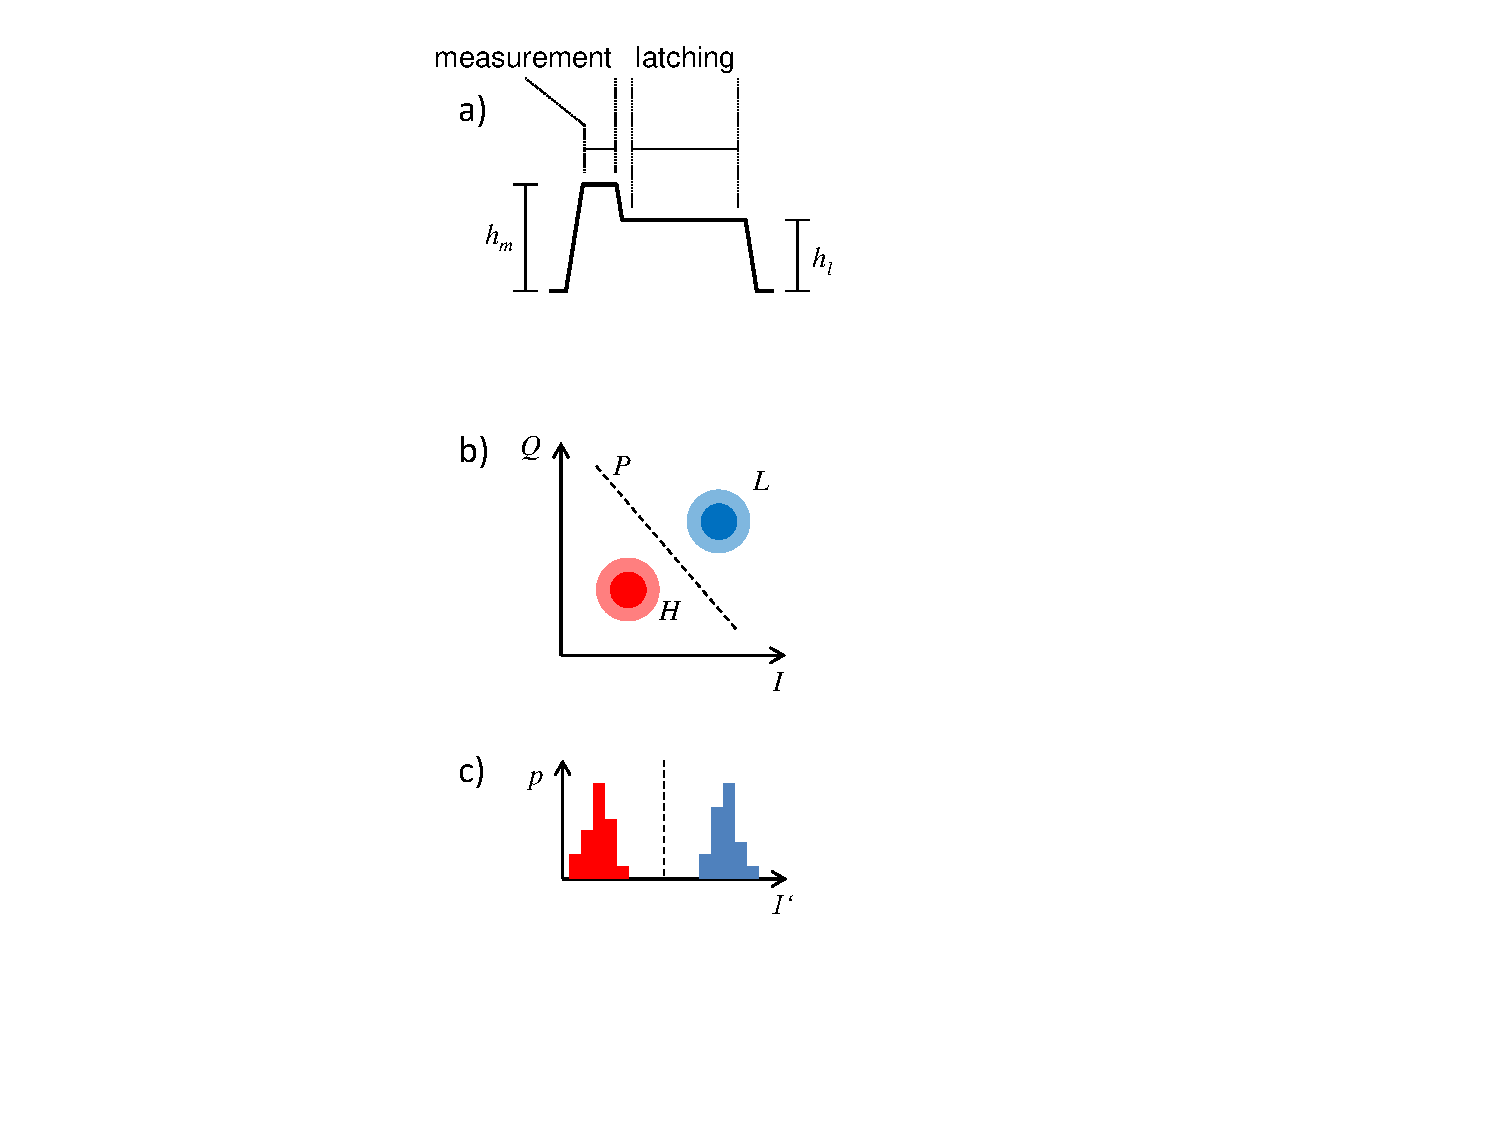
\includegraphics[width=\textwidth]{./material/figures/measurement/readout}
\caption{a) Microwave pulse envelope used for exciting the CJBA during readout. The pulse consists of a measurement part with amplitude $h_m$ and a latching part with ampliude $h_l<h_m$. To determine the state of the resonator during the latching interval, the phase of the reflected signal is meaused in the time window $t_m$. b) Distribution of the measured average $(I,Q)$ values in the IQ plane. The line $P$ that intersects the average quadratures $(I_0,Q_0)$ provides optimal separation between the two clusters corresponding to the state L and H of the resonator. c) Switching probability histograms corresponding to the distribution of the measured $(I,Q)$ values projected along the axis $\perp P$.}
\label{fig:readout_bringup}
\end{figure}

The general readout principle of the CJBA readout that we use in this work is described in section \ref{section:cjba}. Here we explain how we choose the frequency and drive amplitude working point for the readout. To bring up the readout, we first determine the resonance frequency $f_r$ of the CJBA by reflectometry, with the qubit in state $\ket{0}$ and largely detuned from the resonator. We then choose a relative drive detuning $\Omega>\sqrt{3}$ at which the bistable regime is accessible. Next, we mix a continous drive signal with a drive pulse as shown in fig. \ref{fig:readout_bringup}a. We then attenuate the resulting drive signal using a tunable attenuator at room temperature and send it to the CJBA. The reflected and amplified signal is then demodulated with the continous input drive signal using an IQ demodulator. The resulting I/Q quadrature signals are again amplified and get digitized by an ADC card at a sampling rate of 1 GHz during the time window $t_m$, as indicated in fig. \ref{fig:readout_bringup}a. We then average the digitized I/Q signals over the whole measurement window to obtain a single measurement point in the IQ plane and repeat this sequence a large number of times (typically $10^4$). We then repeat this whole procedure for various values of the input attenuation, each time calculating the estimated variance $\hat{\sigma}_{IQ}^2=\sum\limits_i ((I_i-\bar{I}_i)^2+\sum\limits_i (Q_i-\bar{Q}_i)^2)/n$ of the obtained data sets. When starting with a high attenuation and reducing it, at some point the input power sent to the CJBA will be sufficient to make it switch from the L to the H state, thereby changing the phase and consequently the average position of the I/Q values of the obtained signal. Since the switching is a stochasic process, we will observe two families of points close to the transition power. At an input power where approximately 50 \% of switching occurs, the variance $\sigma_{IQ}^2$ of the obtained IQ data points will be largest, as shown in fig. \ref{fig:readout_bringup}b. At this point, we can substract the averages $(I_0=\sum\limits_i I_i / n,Q_0 = \sum\limits_i Q_i/n)$ from the data and perform a principal axis transformation, which diagonalizes the covariance matrix
%
\begin{equation}
\mathrm{var}_{IQ} = \left(\begin{array}{cc}\mathrm{var}(I) & \mathrm{cov}(I,Q) \\ \mathrm{cov}(I,Q) & \mathrm{var}(Q) \end{array}\right)
\end{equation}
%
of the data. Using this transformation, we can project the measured (I,Q) data points on the axis $\perp P$, as shown in fig. \ref{fig:readout_bringup}, and obtain a one-dimensional switching probability distribution. The obtained offsets $I_0$, $Q_0$ and principal axis rotation angle $\alpha_{IQ}$ gives us then the discrimination criterion $Q_L<Q_0+\tan{\alpha_{IQ}}(I-I_0)$ that we can use to classify new data points as belonging to the L or H state at the chosen working point. Normally, if the measurement window $t_m$ is large enough and no retrapping occurs during the meausurement, the distributions corresponding to the L and H states will not overlap, yielding perfect discrimination between them.

\begin{SCfigure}[1][ht!]
\centering
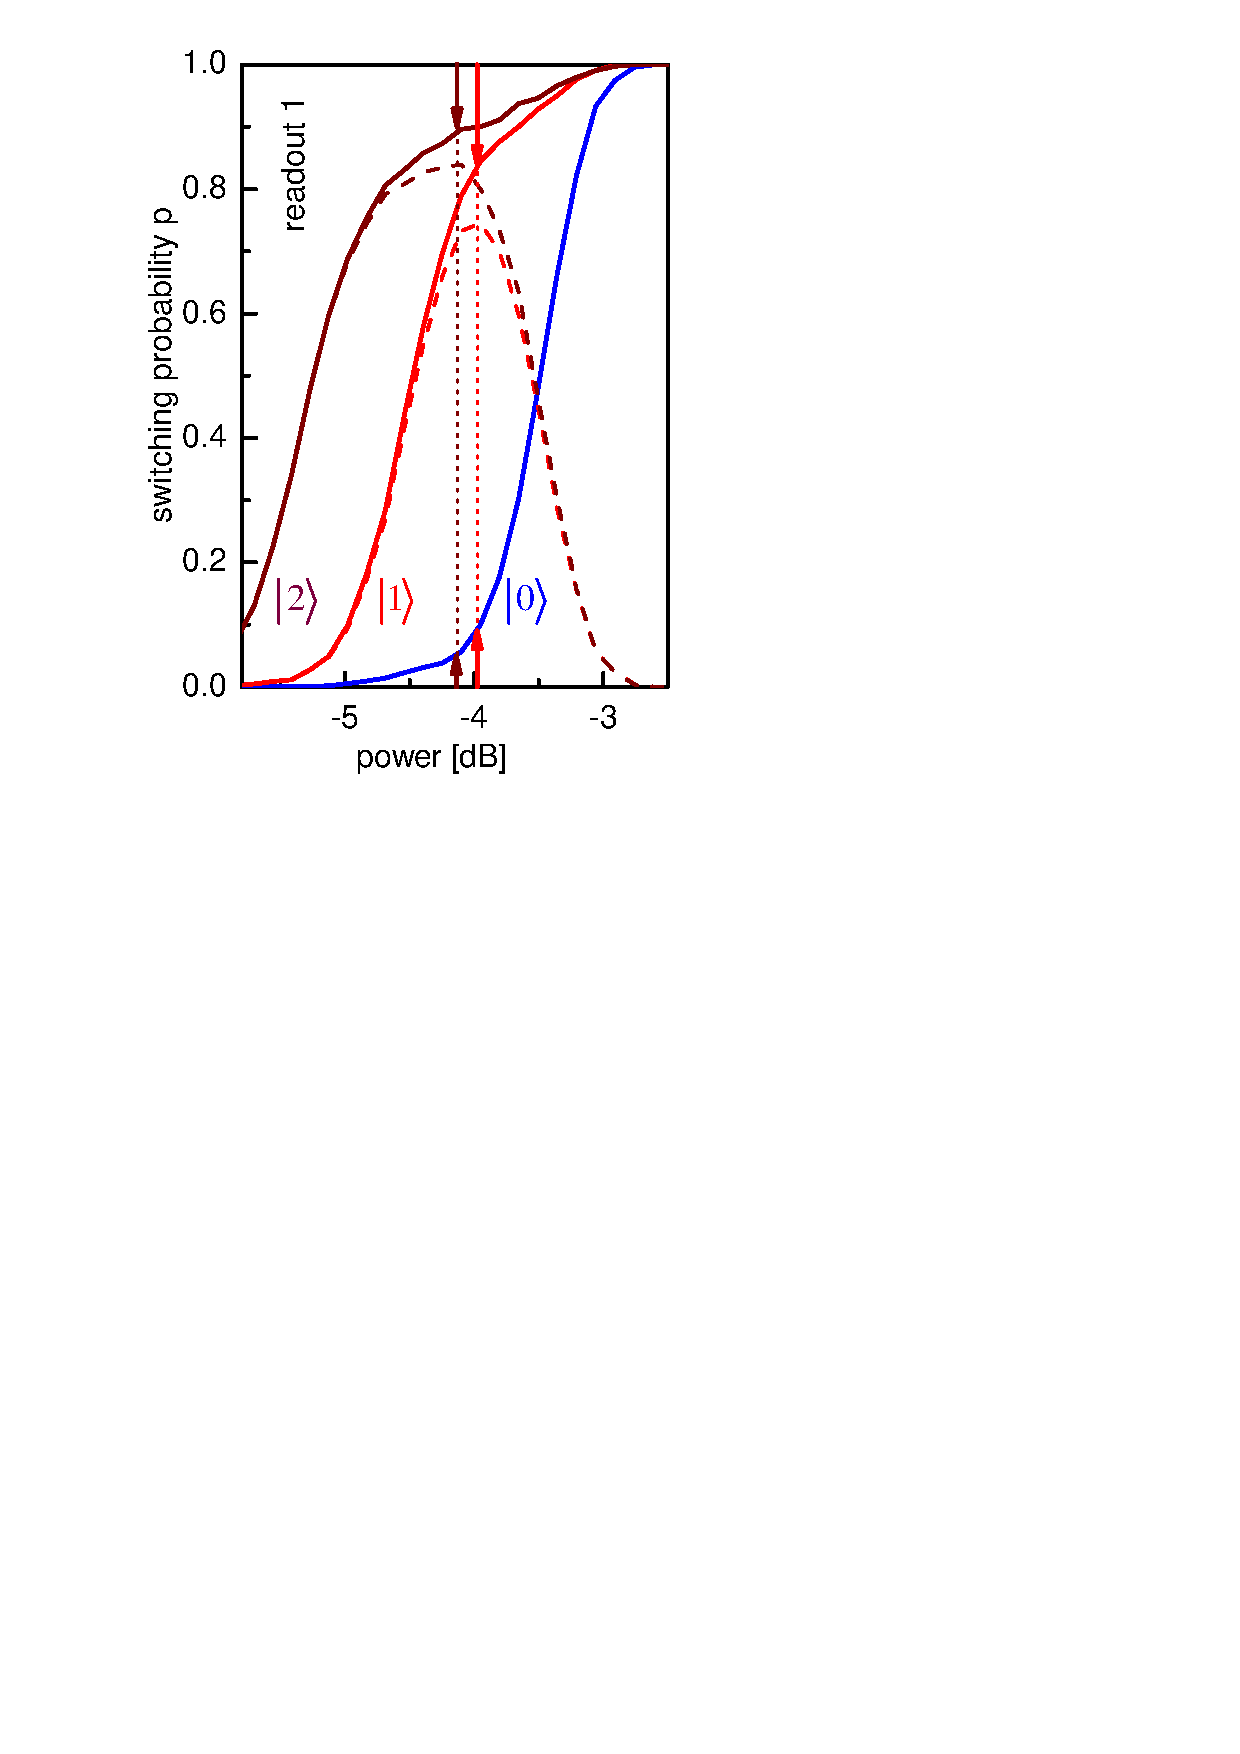
\includegraphics[width=0.4\textwidth]{./material/papers/grover/figures/s_curves_example}
\caption{Exemplary s-curve measurement for one of the qubits on the chip. Shown is the switching probability $p$ of the CJBA as a function of the readout signal power, plotted for different qubit states $\ket{0}$,$\ket{1}$ and $\ket{2}$. The readout contrast between different states is given as the probability difference between the associated switching probability curves. Light and dark red arrows indicate the optimal working points for the $c_{01}$ and $c_{02}$ readout contrasts, respectively.}
\label{fig:s_curves_example}
\end{SCfigure}

\smallskip

After having determined the $I_0$, $Q_0$ and $\alpha_{IQ}$, we slightly tune the attenuation such that we obtain $\approx 20\%$  of switching. At this working point, the readout contrast of the CJBA is usually already sufficient to perform a simple qubit spectroscopy, as described in section \ref{section:qubit_spectroscopy} and calibrate a $X_\pi$ Rabi pulse, as described in section \ref{section:qubit_rabi}. After having done this, we can measure the switching probability of the CJBA readout as a function of the input power while either leaving the qubit in state $\ket{0}$ or exciting it to the state $\ket{1}$. Fig. \ref{fig:s_curves_example} shows an example of such a measurement. Here, the difference $c_{01}$ between the two curves corresponding to the $\ket{1}$ and $\ket{0}$ states corresponds to the input-power dependent readout contrast and allows us to choose the optimum input power for the qubit readout. If desired, we can also perform a $X_\pi^{10}\cdot X_\pi^{12}$ pulse sequence on the qubit to bring it into the state $\ket{2}$ before the readout. In this state, the dispersive shift of the resonator frequency is larger than in the state $\ket{1}$, therefore resulting in a maximum readout contrast $\mathrm{max}(c_{02})>\mathrm{max}(c_{01})$, as shown in fig. \ref{fig:s_curves_example}, which is advantageous when performing e.g. single-run quantum algorithms on the processor, as described in chapter \ref{chapter:grover_algorithm}.

\section{Qubit Manipulation}

To drive the qubits, we need to generate fast microwave pulses with a well defined frequency and phase. As described in one of the previous paragraphs we can use IQ sideband mixing to shape arbitrary drive pulses of the form
%
\begin{equation}
u(t) = I(t)\cos{\omega_{LO}t}+Q(t)\sin{\omega_{LO}t}
\end{equation}
%
We can rewrite this as a product of two complex quantities
%
\begin{equation}
u(t) = \Re\left[ A(t)\cdot\exp{\left(-i\omega_{LO} t\right)}\right].
\end{equation}
%
The X axis of each qubits Bloch sphere is defined by the reference phase of the microwave pulse and can be chosen arbitrarily but must be conserved during one single experimental run. In addition, when performing experiments on multiple qubits, the phase differences between the reference phases of individual qubit drive signals must be conserved between individual runs of the experiment. Thus, to realize a rotation of the qubit state in the XY-plane of the Bloch sphere around an axis $\cos{\phi}\vec{X}+\sin{\phi}\vec{Y}$, we can use a Gaussian-shaped pulse of the form
%
\begin{equation}
A(t) = A_0\cdot\exp{\left(-\frac{(t-t_0)^2}{2\sigma_t}\right)}\cdot\exp{\left(-i\phi\right)}
\end{equation}
%
Here, we typically use a pulse rise time $\sigma_t=3\;\mathrm{ns}$. The advantage of using Gaussian pulses is that the Fourier transform of the pulse is again a Gaussian and, in contrast to a rectangular pulse, does not exhibit side lobes in the frequency domain \citep{bauer_gaussian_1984}. Whenever possible, we just change the height of this pulse to tune the Rabi angle of a given drive pulse. However, for large Rabi angles this is not possible, hence in that case we simply add a flat plateau to the top of the Gaussian pulse. In the following sections we explain how we use such microwave drive pulses to perform qubit spectroscopy, Rabi oscillations and decoherence time measurements.

\subsection{Spectroscopic Measurements of the Qubit State} \label{section:qubit_spectroscopy}

\begin{figure}[ht!]
\centering
a)\includegraphics[width=0.6\textwidth]{"./material/figures/measurement/qubit_spectroscopy"}
b)\includegraphics[width=0.6\textwidth]{"./data/ct5/2011_04_21 - grover and tomo/example - qubit 2 spectroscopy"}
\caption[]{a) Qubit drive and readout pulse sequence used for performing qubit spectroscopy. b) Example of a measured qubit spectroscopy. Shown is the switching probability of the qubit readout when driving the qubit with a very long drive pulse (typically 1 $\mu$s) at a given drive frequency. The resonance to the right (red data points) corresponds to the $\ket{0}\to\ket{1}$ transition of the qubit at frequency $f_{01}$, the resonance on the left (blue data points) to the 2-photon $\ket{0}\to\ket{2}$ transition at frequency $f_{02}/2$. We fit of the two resonances with a Lorentzian to obtain an estimate of the transition frequencies.}
\label{fig:qubit_spectroscopy_example}
\end{figure}

In order to characterize the transition frequency and anharmonicity of the qubit we perform spectroscopic measurements of the qubit state. For this we drive the qubit with a very long Rabi pulse (usually $> 500\;\mathrm{ns}$) at a frequency $\omega_d$. When the drive frequency $\omega_{d}$ is close to the $\omega_{01}$ frequency of the qubit, the drive pulse will induce a Rabi oscillation of the quantum state of the qubit. The induced rotation amplitude will be largest at $\omega_d=\omega_{01}$, Due to decoherence of the qubit during the driven evolution, the maximum probability for measuring the qubit in the state $\ket{1}$ after the pulse is limited to 50 \%. Furthermore, if the drive frequency is sufficiently far detuned from the qubit transition frequency such that $|\omega_d-\omega_{01}|\gg \Gamma^\phi$, no oscillation will be induced and hence the qubit will remain in the state $\ket{0}$. By repeating the pulse sequence shown in fig. \ref{fig:qubit_spectroscopy_example}a for a range of drive frequencies $\omega_d$, a full spectroscopy of the qubit can be obtained. Fig. \ref{fig:qubit_spectroscopy_example}b shows an example of this, where we show the probability of measuring the qubit in state $\ket{1}$ after applying a $1\;\mathrm{\mu s}$ Rabi pulse, plotted as a function of $\omega_d$ and shown for two different drive amplitudes. Here, the blue curve has been measured at $10\;\mathrm{dB}$ higher power than the red curve and shows the two-photon $\ket{0}\to\ket{2}$ transition of the qubit, which can be excited at sufficiently high drive power. By fitting the two resonance curves with a Lorentzian model we obtain the qubit frequencies $f_{01}$ and $f_{02}/2$ and thus the charging and Josephson energies of the qubit at the given working point.

\subsection{Rabi Oscillations} \label{section:qubit_rabi}

\begin{figure}[ht!]
\centering
a)\includegraphics[width=0.6\textwidth]{"./material/figures/measurement/qubit_rabi_oscillation"}
b)\includegraphics[width=0.6\textwidth]{"./data/ct5/2011_04_21 - grover and tomo/example - qubit 2 rabi"}
\caption[]{Example of a measured qubit Rabi experiment. Shown is the switching probability of the qubit readout when driving the qubit at $f_{01}$ with a Gaussian drive pulse of varying duration. The measurement results are not corrected for readout errors.}
\label{fig:qubit_rabi_example}
\end{figure}

After having obtained the proper qubit transition frequency $f_{01}$ using the technique described above, we can perform a Rabi oscillation experiment by driving the qubit for a well-defined time with a drive pulse at the $f_{01}$ transition frequency and measuring the state of the qubit directly afterwards. Figure \ref{fig:qubit_rabi_example}a shows the pulse sequence that we use for a Rabi experiment and fig. \ref{fig:qubit_rabi_example}b shows the resulting measurement data, plotting the readout switching probability as a function of the Rabi drive time. The blue points correspond to measured data whereas the continuous red line corresponds to a fit of a model of the form $p(t)=p_0+a\cos{(\Omega t)}\exp{(-\Gamma_1 t)}$ to the experimental data. As can be seen, the amplitude of the Rabi oscillations gets damped the longer the drive pulse becomes, which is due to relaxation and dephasing during the driven evolution of the qubit. Also, the maximum readout contrast is limited due to readout errors, as we explain in more detail in the following chapter. From the fit of the Rabi data we obtain the Rabi frequency $\Omega$, which we can then use to perform precise single-qubit rotations, as will be explained later. Due to the finite anharmonicity of the qubit, there will always be a leakage to the second excited state $\ket{2}$ of the qubit which gets the more relevant, the faster we drive the system. This leakage mechanism can be an important source of errors and very relevant to the experiments that we discuss later.

\section{Dephasing Time Measurement}

\begin{figure}[ht!]
\centering
a)\includegraphics[width=0.6\textwidth]{"./material/figures/measurement/qubit_ramsey_oscillation"}
b)\includegraphics[width=0.6\textwidth]{"./data/ct5/2011_04_21 - grover and tomo/example - qubit 2 ramsey"}
\caption[]{Example of a measured qubit Ramsey experiment. Shown is the switching probability of the qubit readout after performing a $X_{\pi/2}$-wait-$X_{\pi/2}$ drive sequence at a frequency $f_{01}-\delta f$. Fitting the resulting curve with an attenuated sine-wave model allows us to determine the $f_{01}$ frequency of the Qubit with high accuracy.}
\label{fig:qubit_ramsey_example}
\end{figure}

After having obtained the transition frequency $f_{01}$ of the qubit and the Rabi frequency $\Omega$, we can characterize the dephasing of the qubit by performing a so-called {\it Ramsey fringe experiment}. In this kind of experiment, we first perform a $Y_{\pi/2}$ rotation of the qubit from the state $\ket{0}$, obtaining thus a superposed qubit state of the form $1/\sqrt{2}(\ket{0}+\ket{1})$. Then we displace the qubit frequency by an amount $\Delta f$ by using e.g. a fast magnetic flux pulse and then let the qubit state evolve freely during a certain amount of time $\Delta t$. Finally, we apply another $Y_{\pi/2}$ pulse to the qubit and measure the state of the qubit directly afterwards. The experimental pulse sequence of this experiment is shown in fig. \ref{fig:qubit_ramsey_example}a. Since the qubit frequency relative to the drive reference frame has been deplaced during the free evolution, the qubit will acquire a phase $\Delta \phi = 2\pi\Delta f \Delta t$. The final state of the qubit after applying the second $Y_{\pi/2}$ pulse will therefore become
%
\begin{equation}
\ket{\phi_f} = \left(\begin{array}{cc} 1 & -1 \\ 1 & 1 \end{array} \right)\cdot\left(\begin{array}{c} 1 \\ e^{i\Delta\phi} \end{array}\right) = \left( \begin{array}{c} i\sin{\Delta\phi/2} \\ -\cos{\Delta\phi/2}\end{array}\right)
\end{equation}
%
Hence, the resulting state $\ket{\phi_f}$ will oscillate between the state $\ket{0}$ and $\ket{1}$ as a function of the delay with a frequency $\Delta f/2$. As before, due to dephasing and relaxation during the free evolution of the qubit state, the amplitude of these oscillations will decay. If the system dephasing time is limited by qubit relaxation, the decay will follow a Gaussian of the form $\exp{(-\Gamma t^2)}$, otherwise it will also exhibit an exponential decay $\simeq \exp{(-\Gamma t)}$. In the Ramsey sequence, instead of detuning the qubit frequency during the free evolution phase we can also simply detune the qubit drive frequency instead, thereby changing the drive reference frame instead of the real qubit frequency. If this detuning is small in comparision to the Rabi frequency $\Omega$, we will still be able to accurately perform the first $Y_{\pi/2}$ pulse. However, since the drive reference frequency is now slighty detuned from that of the qubit, the state in the drive reference frame will acquire a relative phase $\Delta f \Delta t$ during the free evolution phase. By fitting the experimental data obtained for such an experiment to a model of the form $p(\ket{1}) = p_0 +a\cos{(\Delta f \Delta t+\phi_0)}\exp{(-\Gamma_2 t^2/2)}$ we can obtain an estimate of $\Delta f$ and $\Gamma_2$, thereby characterizing the effective dephasing time of the qubit. Fig. \ref{fig:qubit_ramsey_example}b shows an example of measured Ramsey data with a corresponding fit. Furthermore, since we know the frequency detuning of the drive during the free evolution of the qubit we can substract it from the fitted value $\Delta f$ and obtain the residual detuning of the qubit frequency from the drive frequeny. This allows us to precisely determine the qubit frequency and to correct drive frequency errors with an accuracy of typically $100\;\mathrm{kHz}$. 

\section{Relaxation Time Measurement}

\begin{figure}[ht!]
\centering
a)\includegraphics[width=0.6\textwidth]{"./material/figures/measurement/qubit_t1_measurement"}
b)\includegraphics[width=0.6\textwidth]{"./data/ct5/2011_04_21 - grover and tomo/example - qubit 2 t1"}
\caption[]{Example of a qubit relaxation time measurement. Shown is the probability of measuring the qubit in state $\ket{1}$ as a function of the delay time between the preparation of the state $\ket{1}$ and the actual measurement of the qubit state. The decay of this probability follows an exponential law of the form $p(\ket{1})\simeq\exp{(-\Gamma_1 t)}$}
\label{fig:qubit_t1_example}
\end{figure}

We can characterize the relaxation time of the qubit by performing a simple experiment where we put the qubit in state $\ket{1}$ by applying a $X_{\pi}$ pulse and let it evolve freely afterwards for a given time before reading out its state, as shown in fig. \ref{fig:qubit_t1_example}a. Due to coupling of the qubit to its environment, relaxation to the ground state can occur during the free evolution. Hence, the longer we wait, the higher the probability that the qubit has relaxed to the ground state. An example of the resulting probability curve obtained through such an experiment is shown in fig. \ref{fig:qubit_t1_example}b. It shows the probability of measuring the qubit in state $\ket{1}$, plotted as a function of the delay between the initial state preparation and the measurement of its state. As can be seen, the probability decreases exponentially as a function of time. As before, in the curve the blue markers correspond to experimental data and the red line corresponds to a fit of this data to a model of the form $p(\ket{1}) = p_0+p_a\exp{(-\Gamma_1 t)}$. From this fit, we can then extract the relaxation rate $\Gamma_1$ of the qubit at the given working point. In the following chapter we will look more in detail at the relaxation time of both qubits of our processor as a function of their transition frequency and their detuning from the readout resonator.